\subsection{Cartes \emph{Arduino Mega}}

\subsubsection{Matériel utilisé}

Le deuxième type de cartes que nous devions utiliser était l’\emph{Arduino Mega} 2560 (\cref{arduino}).

\begin{figure}[H]
\centering
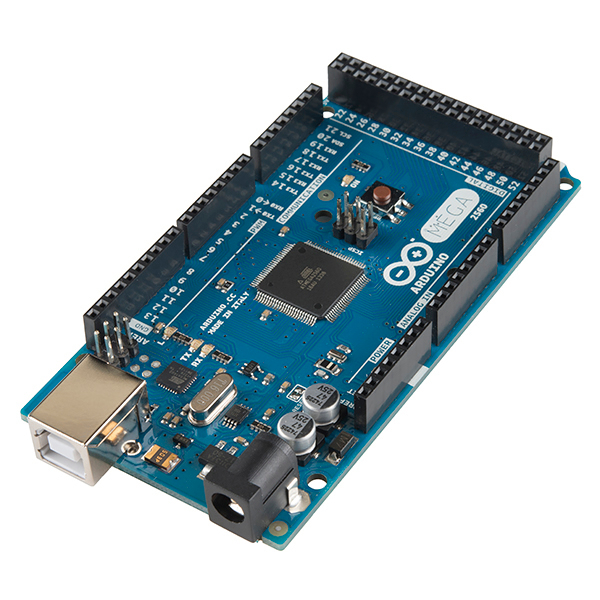
\includegraphics[width=8cm]{\rpDossier/images/arduino.jpg}
\caption{Carte \emph{Arduino Mega}}
\label{arduino}
\end{figure}

La communication sans fil n’est pas intégrée à cette carte \emph{Arduino}, contrairement à la CC 2538, aussi avons-nous utilisé une puce \emph{XBee} (\cref{xbee}), ainsi qu’une carte d’adaptation (à droite de la \cref{xbee-shields}).

\begin{figure}[H]
\centering
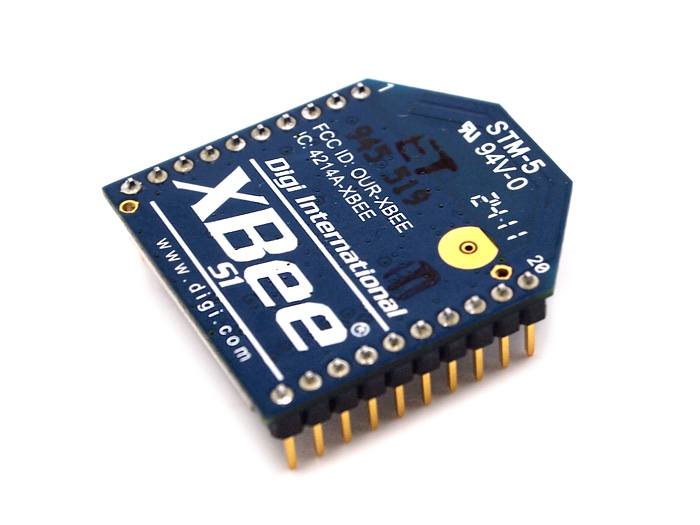
\includegraphics[width=5cm]{\rpDossier/images/xbee.jpg}
\caption{Puce \emph{XBee}}
\label{xbee}
\end{figure}

La carte d’adaptation que nous avons utilisée n’est pas la même que celle utilisée dans l’étude que nous devions reproduire \cite{eymery}, produite par \emph{Arduino} (à gauche de la \cref{xbee-shields}).

\begin{figure}[H]
\centering
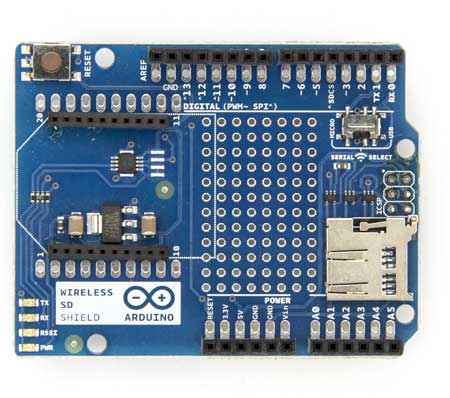
\includegraphics[height=6cm]{\rpDossier/images/arduino-shield.jpg}
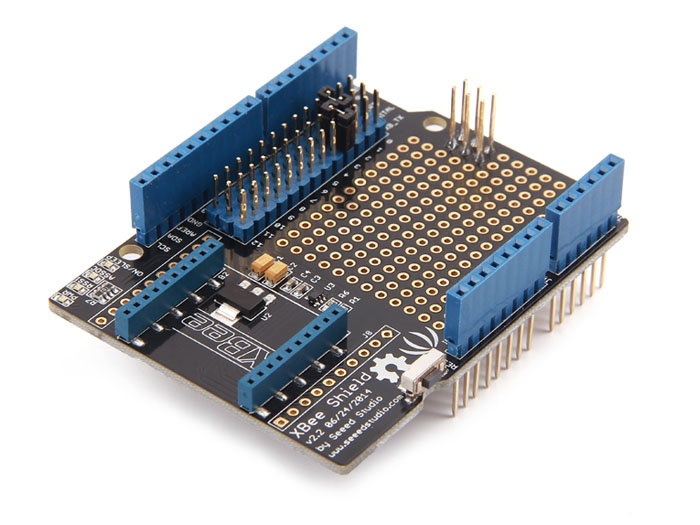
\includegraphics[height=6cm]{\rpDossier/images/xbee-shield.jpg}
\newline
À gauche la carte d’\emph{Arduino}, à droite celle de \emph{Seeed Studio}.
\caption{Cartes d’adaptation pour puce \emph{XBee}}
\label{xbee-shields}
\end{figure}

\subsubsection{Outils de développement}

\paragraph{Environnement de développement}

Les cartes \emph{Arduino} sont accompagnées d’un environnement de développement intégré spécifique \cref{arduino-ide}.
En plus de la compilation et le téléchargement des programmes sur la carte, celui-ci propose notamment une console permettant de consulter le flux de sortie standard des cartes.

\begin{figure}[H]
\centering
\todo[Copie d’écran de l’IDE]
\caption{Environnement de développement d’\emph{Arduino}}
\label{arduino-ide}
\end{figure}

\paragraph{Pile 6LoWPAN}

Pour la communication 6LoWPAN, nous devions utiliser une bibliothèque qui a été adaptée par \emph{Télécom Bretagne} à partir de l’implémentation \emph{sicslowpan} qui est utilisée dans \emph{Contiki} \citeweb{sicslowpan-telecom}.

Le code de l’exemple inclus dans cette bibliothèque a été conçu pour la carte produite par \emph{Arduino} : il nécessite la modification des branchements de la carte d’adaptation après le téléchargement du programme, afin de laisser le canal de communication série libre pour les communications avec la puce \emph{XBee}.
Nous avons pu le comprendre en comparant les caractères envoyés dans le flux de sortie standard (grâce à la console) et les séquences de contrôle de la carte \emph{XBee}
La carte produite par \emph{Arduino} dispose d’un petit bouton qui permet de faire ce changement de branchement aisément, mais pas la carte dont nous disposions : sur celle-ci, le branche permet des configurations plus avancées est effectué en déplaçant un cavalier sur trois rangées de broches.

Un des \textit{forks} de la bibliothèque \citeweb{sicslowpan-chuljin} semble avoir été modifié pour pouvoir utiliser d’autres broches que celles par défaut et donc profiter de cette plus grande capacité d’adaptation : il permet de définir un objet \textit{SoftwareSerial} à la place du \textit{HardwareSerial} qui est limité aux broches de la sortie par défaut.
Le temps nous manquait et nous avons décidé avec notre tuteur de nous concentrer sur les CC 2538.
Nous n’avons par conséquent pas exploré les possibilités de cette version de la bibliothèque.


